\section{Stjärnornas anatomi}
En stjärna är i grund och botten en boll av gas. Först och främst består dem av väte (\chemfig{H}) och helium (\chemfig{He}). De innehåller dock ämnen hela vägen upp till järn (\chemfig{Fe}) periodiska systemet (se \cref{fig:periodic-table} för ett periodiskt system).

Deras inre struktur kan liknas till en lök. I mitten finns kärnan, sedan har man lager av olika gaser och plasman för att sista komma ut till yttersta skicket av gas som vi ser utifrån. Ett diagram återfinns i \cref{fig:star-anatomy}.

\begin{figure}[hb]
    \centering
    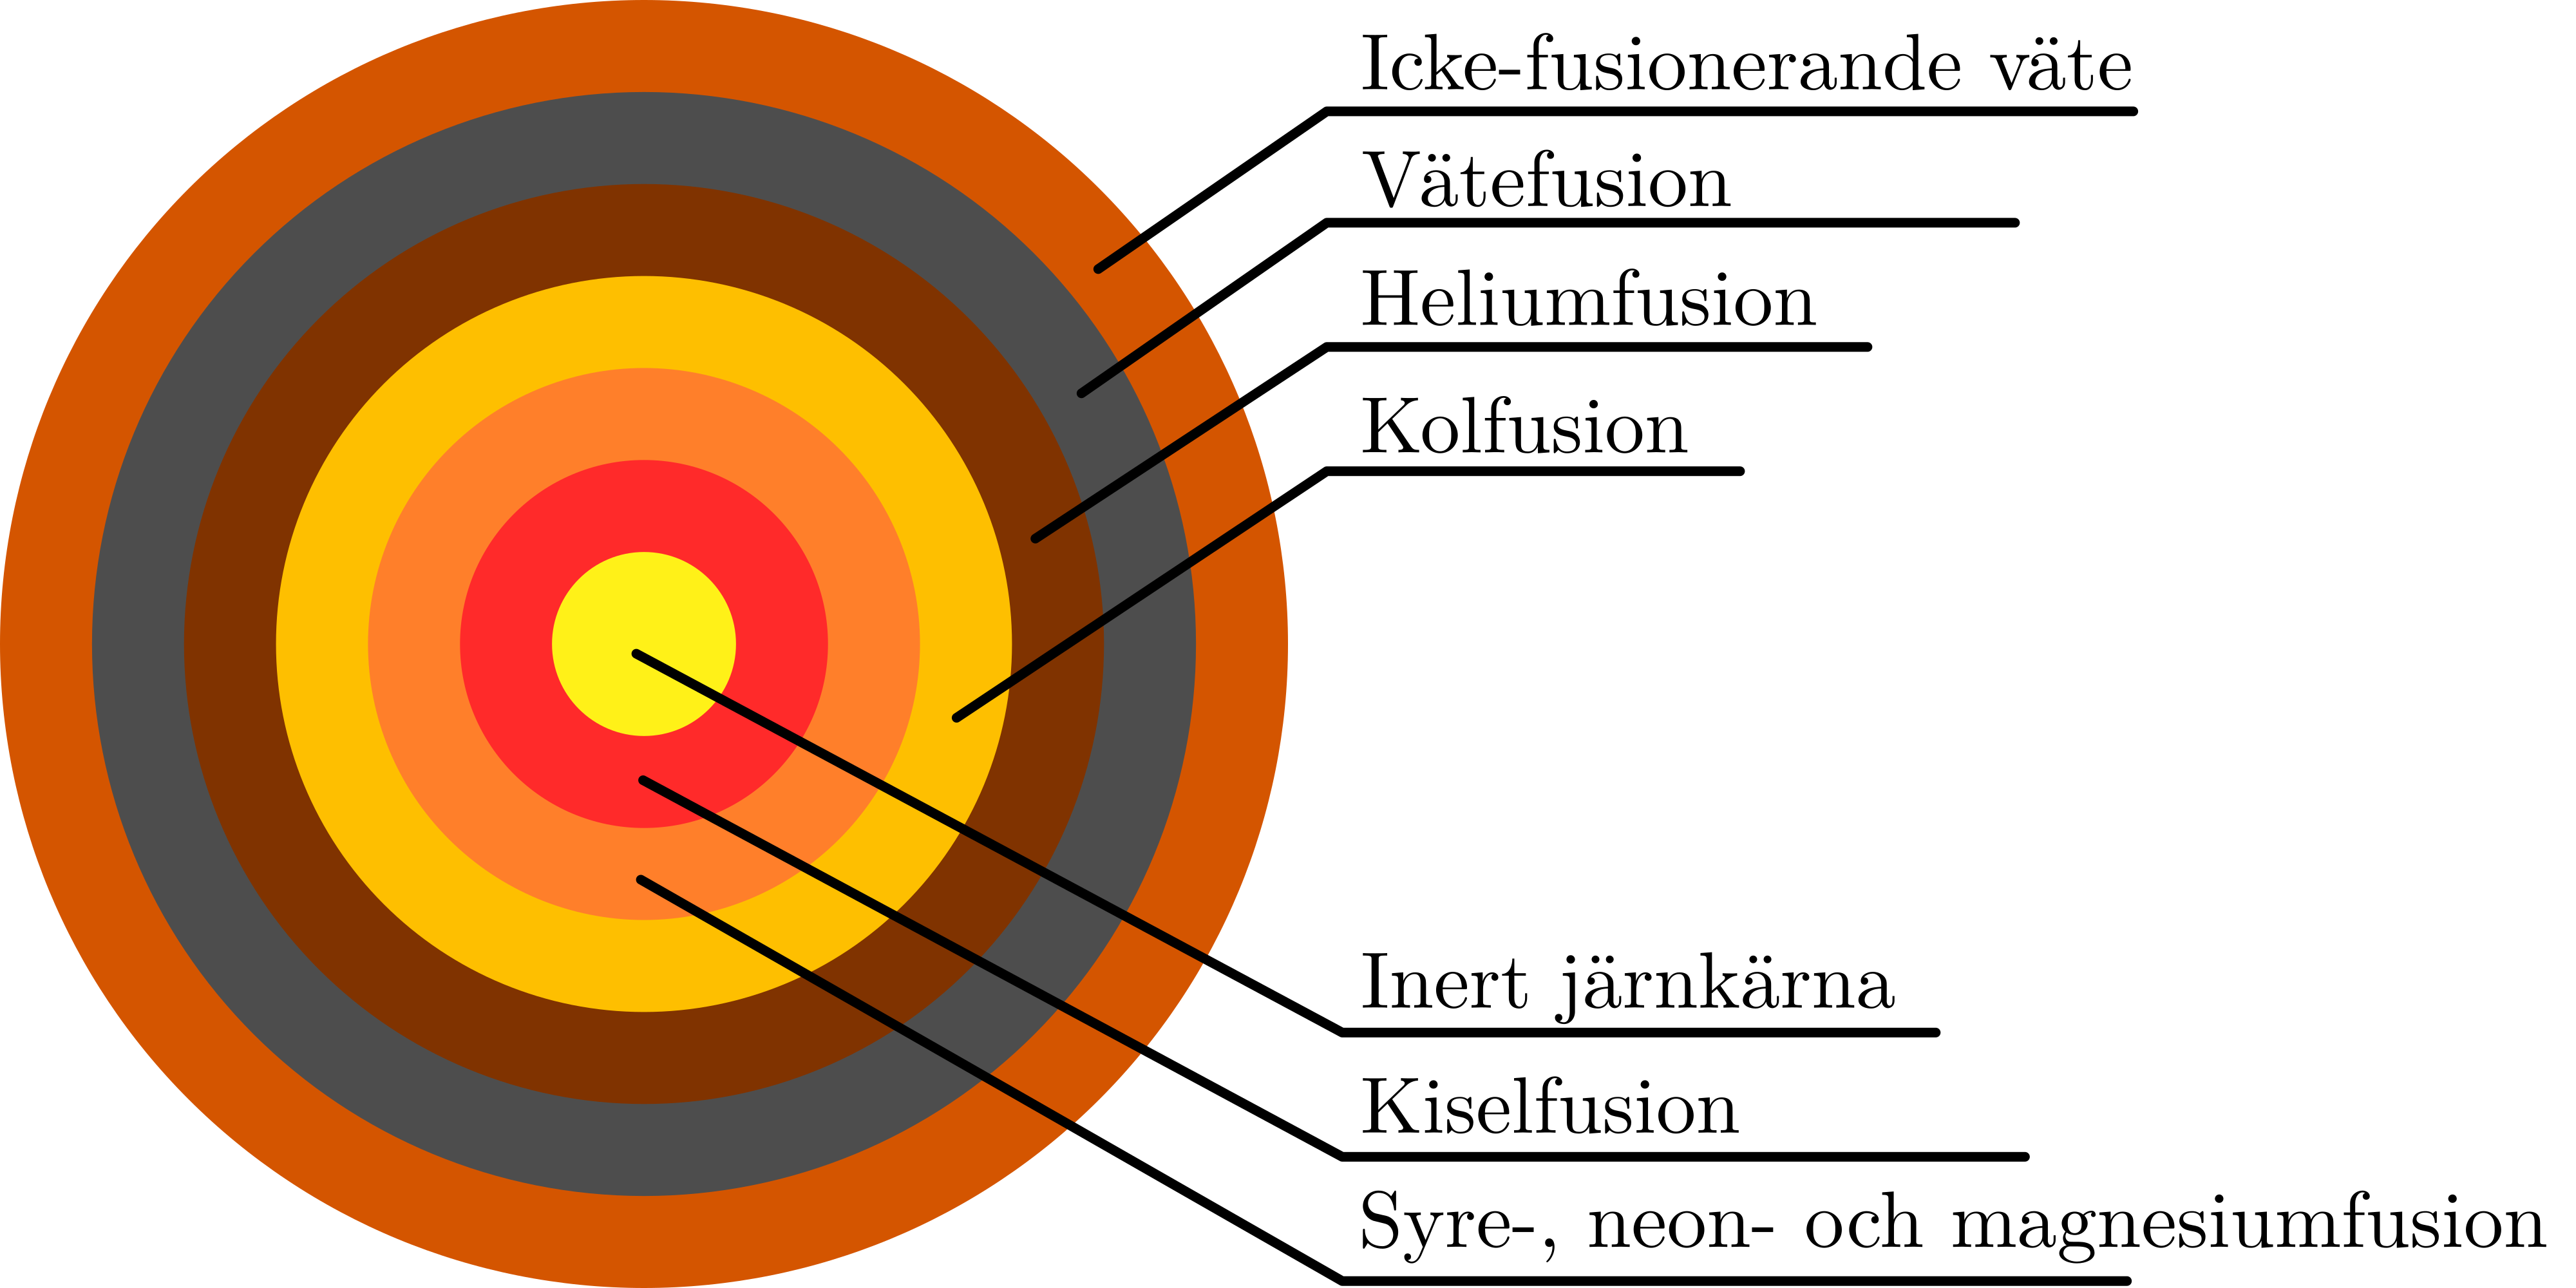
\includegraphics[width=0.8\textwidth]{img/star.png}
    \caption{En gammal stjärnas inre struktur.}
    \label{fig:star-anatomy}
\end{figure}